\documentclass[11pt,a4paper]{article}

% ---------------------------------------------------------------------------
% Encodage, langue et typographie
% ---------------------------------------------------------------------------
\usepackage[utf8]{inputenc}
\usepackage[T1]{fontenc}
\usepackage[french]{babel}
\usepackage{tgpagella}
\usepackage{tgheros}
\usepackage[scaled=0.85]{beramono}
\usepackage{textcomp}
\usepackage{microtype}
\usepackage{parskip}
\setlength{\parskip}{0.45em}

% ---------------------------------------------------------------------------
% Mise en page
% ---------------------------------------------------------------------------
\usepackage[a4paper,top=2.4cm,bottom=2.4cm,left=2.5cm,right=2.5cm,headheight=22pt]{geometry}
\usepackage{fancyhdr}
\usepackage{setspace}
\setstretch{1.08}

\usepackage[table]{xcolor}
\definecolor{coverblue}{HTML}{1F3A5F}
\definecolor{teal}{HTML}{0F766E}
\definecolor{accent}{HTML}{D97706}
\definecolor{lightbg}{HTML}{F1F5F9}
\definecolor{codebg}{HTML}{F8FAFC}
\definecolor{codeblue}{HTML}{1D4ED8}
\definecolor{codecomment}{HTML}{64748B}
\definecolor{codestring}{HTML}{B91C1C}
\definecolor{codegray}{HTML}{94A3B8}

\usepackage{graphicx}
\usepackage{float}
\usepackage{booktabs}
\usepackage{tabularx}
\usepackage{array}
\usepackage{enumitem}
\usepackage{caption}
\usepackage{titlesec}
\usepackage{tikz}
\usetikzlibrary{positioning,arrows.meta,shapes.geometric,calc,fit,backgrounds}
\usepackage{pgfplots}
\pgfplotsset{compat=1.18}
\usepackage[most]{tcolorbox}
\usepackage{listings}
\usepackage{fontawesome5}

\usepackage[colorlinks=true,linkcolor=coverblue,urlcolor=teal,citecolor=teal,
            pdftitle={Smart Room Monitoring - Rapport d'atelier IoT},
            pdfauthor={Youssef El Ajbari}]{hyperref}

% ---------------------------------------------------------------------------
% En-tetes et pieds de page
% ---------------------------------------------------------------------------
\pagestyle{fancy}
\fancyhf{}
\fancyhead[L]{\small\sffamily\color{coverblue}\nouppercase{\leftmark}}
\fancyhead[R]{\small\sffamily\color{coverblue}Atelier 6 --- IoT}
\fancyfoot[C]{\small\sffamily\color{gray}Page \thepage}
\renewcommand{\headrulewidth}{0.4pt}
\renewcommand{\headrule}{\hbox to\headwidth{\color{teal}\leaders\hrule height \headrulewidth\hfill}}
\fancypagestyle{plain}{%
  \fancyhf{}%
  \fancyfoot[C]{\small\sffamily\color{gray}Page \thepage}%
  \renewcommand{\headrulewidth}{0pt}%
}

\renewcommand{\sectionmark}[1]{\markboth{\thesection.\ #1}{}}

% ---------------------------------------------------------------------------
% Titres
% ---------------------------------------------------------------------------
\titleformat{\section}
  {\Large\bfseries\color{coverblue}}
  {\thesection}{0.7em}{}
\titlespacing*{\section}{0pt}{1.3ex plus .2ex}{0.9ex plus .1ex}

\titleformat{\subsection}
  {\large\bfseries\color{teal}}
  {\thesubsection}{0.6em}{}
\titlespacing*{\subsection}{0pt}{1.0ex plus .1ex}{0.5ex plus .1ex}

\titleformat{\subsubsection}
  {\normalsize\bfseries\color{coverblue}}
  {\thesubsubsection}{0.5em}{}
\titlespacing*{\subsubsection}{0pt}{0.8ex plus .1ex}{0.3ex}

% ---------------------------------------------------------------------------
% Legendes, listes, tableaux
% ---------------------------------------------------------------------------
\captionsetup{font=small,labelfont={bf,color=coverblue},justification=centering,skip=5pt}
\captionsetup[table]{position=top,skip=4pt}
\renewcommand{\arraystretch}{1.22}
\setlist[itemize]{leftmargin=1.5em,itemsep=2pt,topsep=4pt,parsep=0pt}
\setlist[enumerate]{leftmargin=1.8em,itemsep=2pt,topsep=4pt,parsep=0pt}

% ---------------------------------------------------------------------------
% Code source
% ---------------------------------------------------------------------------
\lstdefinelanguage{JavaScript}{
  keywords={break,case,catch,const,continue,debugger,default,delete,do,else,
            export,extends,finally,for,function,if,import,in,instanceof,let,
            new,return,super,switch,this,throw,try,typeof,var,void,while,with,
            yield,async,await,class,of,static,get,set,true,false,null,undefined},
  sensitive=true,
  comment=[l]{//},
  morecomment=[s]{/*}{*/},
  morestring=[b]',
  morestring=[b]",
  morestring=[b]`
}

\lstset{
  backgroundcolor=\color{codebg},
  basicstyle=\ttfamily\footnotesize,
  keywordstyle=\color{codeblue}\bfseries,
  commentstyle=\color{codecomment}\itshape,
  stringstyle=\color{codestring},
  numbers=left,
  numberstyle=\tiny\color{codegray},
  numbersep=8pt,
  xleftmargin=1.6em,
  framexleftmargin=1.2em,
  frame=single,
  framesep=4pt,
  rulecolor=\color{coverblue!22},
  breaklines=true,
  breakatwhitespace=false,
  postbreak=\mbox{\textcolor{codegray}{$\hookrightarrow$}\space},
  showstringspaces=false,
  tabsize=2,
  captionpos=b,
  extendedchars=true,
  inputencoding=utf8,
  aboveskip=8pt,
  belowskip=8pt,
  literate=
    {à}{{\`a}}1 {â}{{\^a}}1 {ä}{{\"a}}1 {ç}{{\c c}}1
    {é}{{\'e}}1 {è}{{\`e}}1 {ê}{{\^e}}1 {ë}{{\"e}}1
    {î}{{\^i}}1 {ï}{{\"i}}1 {ô}{{\^o}}1 {ö}{{\"o}}1
    {ù}{{\`u}}1 {û}{{\^u}}1 {ü}{{\"u}}1 {ÿ}{{\"y}}1
    {œ}{{\oe}}1 {Œ}{{\OE}}1 {À}{{\`A}}1 {É}{{\'E}}1
    {È}{{\`E}}1 {Ê}{{\^E}}1 {Ç}{{\c C}}1 {°}{{\textdegree}}1
    {’}{{'}}1 {–}{{--}}1 {—}{{---}}1 {…}{{\ldots}}1
    {⚠}{{!}}1
}
\renewcommand{\lstlistingname}{Code}
\captionsetup[lstlisting]{font=small,labelfont={bf,color=coverblue},justification=centering}

% ---------------------------------------------------------------------------
% Quelques commandes utiles
% ---------------------------------------------------------------------------
\newcommand{\code}[1]{\texttt{#1}}
\newcommand{\figref}[1]{\figurename~\ref{#1}}
\newcommand{\tabref}[1]{\tablename~\ref{#1}}
\newcommand{\coderef}[1]{\lstlistingname~\ref{#1}}

\newcommand{\objectifs}{%
\begin{tcolorbox}[colback=teal!5,colframe=teal,coltitle=white,
  title={\bfseries Objectifs de l'atelier},arc=3pt,boxrule=0.8pt,
  left=7pt,right=7pt,top=5pt,bottom=5pt]
\begin{itemize}
  \item acquérir la température et l'humidité avec un capteur DHT22 ;
  \item transmettre les mesures en Wi-Fi vers un serveur avec un protocole HTTP et un format JSON ;
  \item développer un serveur Node.js qui valide, mémorise et rediffuse les mesures en temps réel ;
  \item concevoir un tableau de bord web lisible, réactif et doté d'alertes ;
  \item valider la chaîne complète et analyser les résultats expérimentaux.
\end{itemize}
\end{tcolorbox}
}

\begin{document}

% ===========================================================================
% PAGE DE GARDE
% ===========================================================================
\begin{titlepage}
\thispagestyle{empty}
\begin{tikzpicture}[remember picture,overlay]
  % Bandeau superieur
  \fill[coverblue] (current page.north west) rectangle ([yshift=-7.4cm]current page.north east);
  \fill[teal] ([yshift=-7.4cm]current page.north west) rectangle ([yshift=-7.55cm]current page.north east);

  % Cercles decoratifs
  \draw[white,opacity=0.07,line width=1.2mm] ([xshift=2.2cm,yshift=-2.0cm]current page.north west) circle (2.6cm);
  \draw[white,opacity=0.06,line width=1.0mm] ([xshift=16.4cm,yshift=-5.4cm]current page.north west) circle (3.4cm);
  \node[white,opacity=0.13,font=\fontsize{105}{105}\selectfont]
    at ([xshift=15.3cm,yshift=-4.2cm]current page.north west) {\faWifi};

  % Textes du bandeau
  \node[anchor=west,text=white,font=\sffamily\bfseries\large]
    at ([xshift=2.2cm,yshift=-1.45cm]current page.north west) {RAPPORT DE TRAVAUX PRATIQUES};
  \node[anchor=west,text=white,font=\sffamily\large]
    at ([xshift=2.2cm,yshift=-2.15cm]current page.north west) {Internet des objets --- Atelier 6, partie 1};
  \node[anchor=west,text=white,font=\sffamily\bfseries\fontsize{31}{36}\selectfont,text width=14cm,align=left]
    at ([xshift=2.2cm,yshift=-3.65cm]current page.north west) {Smart Room\\Monitoring};
  \node[anchor=west,text=white,font=\sffamily\large]
    at ([xshift=2.2cm,yshift=-6.55cm]current page.north west) {Chaîne IoT complète et supervision temps réel};

  % Sous-titre
  \node[anchor=west,text=coverblue,font=\sffamily\bfseries\Large,text width=15cm,align=left]
    at ([xshift=2.2cm,yshift=-8.55cm]current page.north west)
    {Acquisition DHT22, transmission ESP32,\\serveur Node.js et tableau de bord web};
  \draw[teal,line width=1.2pt] ([xshift=2.2cm,yshift=-10.15cm]current page.north west) -- ++(5.3cm,0);

  \node[anchor=north west,text=black!68,font=\normalsize,text width=13.8cm,align=left]
    at ([xshift=2.2cm,yshift=-10.45cm]current page.north west)
    {Ce rapport présente la conception, la réalisation et la validation d'une chaîne
     d'Internet des objets permettant de mesurer la température et l'humidité d'une salle,
     de transmettre les données à un serveur et de les visualiser en temps réel dans un
     navigateur.};

  % Schema synthetique
  \node[draw=teal,fill=teal!5,rounded corners=4pt,line width=0.8pt,
        text width=14.2cm,align=center,inner sep=10pt,anchor=west]
    at ([xshift=2.2cm,yshift=-13.85cm]current page.north west)
    {\sffamily\bfseries\color{coverblue}DHT22\quad$\rightarrow$\quad ESP32\quad$\rightarrow$\quad
     Node.js / Express\quad$\rightarrow$\quad Socket.IO\quad$\rightarrow$\quad Dashboard};

  % Bloc auteur
  \node[anchor=west,text=black!60,font=\sffamily\small]
    at ([xshift=2.2cm,yshift=-18.1cm]current page.north west) {PRÉSENTÉ PAR};
  \node[anchor=west,text=coverblue,font=\sffamily\bfseries\Large]
    at ([xshift=2.2cm,yshift=-18.75cm]current page.north west) {Youssef El Ajbari et Monssef Bougaidan};
  \node[anchor=west,text=black!75,font=\sffamily\normalsize]
    at ([xshift=2.2cm,yshift=-19.55cm]current page.north west) {3\up{e} année --- IDAI};
  \node[anchor=west,text=black!75,font=\sffamily\normalsize]
    at ([xshift=2.2cm,yshift=-20.15cm]current page.north west) {Module : Internet des objets};
  \node[anchor=west,text=black!75,font=\sffamily\normalsize]
    at ([xshift=2.2cm,yshift=-21.55cm]current page.north west) {30 octobre 2026};
  \node[anchor=west,text=black!55,font=\sffamily\small]
    at ([xshift=2.2cm,yshift=-22.15cm]current page.north west) {Année universitaire 2026--2027};

  % Bandeau inferieur
  \fill[coverblue] (current page.south west) rectangle ([yshift=2.2cm]current page.south east);
  \fill[teal] ([yshift=2.2cm]current page.south west) rectangle ([yshift=2.32cm]current page.south east);
  \node[text=white,font=\sffamily\small]
    at ([yshift=1.1cm]current page.south) {ESP32 \quad$\cdot$\quad DHT22 \quad$\cdot$\quad HTTP/JSON \quad$\cdot$\quad WebSocket \quad$\cdot$\quad Node.js};
\end{tikzpicture}
\null
\end{titlepage}

% ===========================================================================
% SOMMAIRE
% ===========================================================================
\pagenumbering{roman}
\setcounter{tocdepth}{1}
\renewcommand{\contentsname}{Sommaire}
\tableofcontents
\clearpage

% ===========================================================================
% CORPS DU RAPPORT
% ===========================================================================
\pagenumbering{arabic}
\setcounter{page}{1}

% ---------------------------------------------------------------------------
\section{Introduction}
% ---------------------------------------------------------------------------

\subsection{Contexte}

Les ateliers précédents ont introduit la commande d'une LED, la lecture d'un capteur DHT22
et une première logique locale de \og Smart Room \fg{}. L'atelier 6 change d'échelle : il ne
s'agit plus seulement de faire clignoter une sortie ou d'afficher une mesure sur un écran
local, mais de construire une chaîne complète, depuis le capteur jusqu'à une interface
consultable à distance.

Le système réalisé, nommé \textbf{Smart Room Monitoring}, poursuit un objectif simple :
rendre disponible en temps réel, dans un navigateur, la température et l'humidité d'une salle.
Cette contrainte impose de résoudre plusieurs problèmes complémentaires : acquisition fiable,
transmission réseau, validation des données, stockage temporaire, diffusion événementielle et
présentation ergonomique.

\objectifs

\subsection{Cahier des charges}

Le tableau~\ref{tab:cahier} résume les exigences retenues et les critères d'acceptation
associés. Ces critères ont guidé les choix techniques et servi de base aux essais de la
partie 6.

\begin{table}[H]
\centering
\small
\begin{tabularx}{\textwidth}{@{}>{\bfseries}p{3.1cm} X@{}}
\toprule
Exigence & Critère d'acceptation \\
\midrule
Acquisition & Température et humidité lues automatiquement toutes les 5~s. \\
Transmission & Envoi HTTP POST d'un objet JSON vers \texttt{/api/measurements}, avec réponse 200 en cas de succès. \\
Validation & Rejet par un code 400 des données manquantes, mal typées ou hors plage. \\
Temps réel & Mise à jour du tableau de bord sans rechargement, via Socket.IO. \\
Historique & Conservation et affichage des dix dernières mesures. \\
Alertes & Signalement visuel si la température dépasse 30~\textdegree C ou si l'humidité dépasse 70~\%. \\
Interface & Page responsive, état de connexion visible, horodatage des mesures. \\
\bottomrule
\end{tabularx}
\caption{Cahier des charges fonctionnel de l'atelier.}
\label{tab:cahier}
\end{table}

% ---------------------------------------------------------------------------
\section{Architecture générale}
% ---------------------------------------------------------------------------

\subsection{Vue d'ensemble}

L'architecture suit un modèle en trois couches, représenté sur la figure~\ref{fig:architecture} :

\begin{itemize}
  \item \textbf{couche de perception} : le capteur DHT22 mesure la température et l'humidité,
        l'ESP32 les acquiert et les met en forme ;
  \item \textbf{couche de traitement} : le serveur Node.js reçoit les requêtes HTTP, valide
        les données, les stocke en mémoire et les rediffuse ;
  \item \textbf{couche de présentation} : le navigateur affiche le tableau de bord et reçoit
        les mises à jour par WebSocket.
\end{itemize}

\begin{figure}[H]
\centering
\begin{tikzpicture}[
  node distance=1.0cm and 1.55cm,
  box/.style={draw=coverblue!55,fill=coverblue!5,rounded corners=4pt,
              text width=3.1cm,minimum height=1.8cm,align=center,
              font=\sffamily\small,inner sep=4pt},
  arr/.style={-{Latex[length=2.6mm]},line width=0.9pt,draw=teal},
  lab/.style={font=\scriptsize,fill=white,inner sep=1pt,text=black!70}
]
  \node[box] (sensor) {\faThermometerHalf\\[2pt]\textbf{DHT22}\\[1pt]{\footnotesize Température\\et humidité}};
  \node[box,right=of sensor] (esp) {\faMicrochip\\[2pt]\textbf{ESP32}\\[1pt]{\footnotesize Acquisition\\et Wi-Fi}};
  \node[box,right=of esp] (server) {\faServer\\[2pt]\textbf{Serveur Node.js}\\[1pt]{\footnotesize Express\\et Socket.IO}};
  \node[box,below=1.35cm of server] (browser) {\faDesktop\\[2pt]\textbf{Dashboard web}\\[1pt]{\footnotesize HTML, CSS\\et JavaScript}};

  \draw[arr] (sensor) -- node[above,lab]{GPIO 17} node[below,lab]{données} (esp);
  \draw[arr] (esp) -- node[above,lab]{HTTP POST} node[below,lab]{JSON / 5 s} (server);
  \draw[arr] (server) -- node[right,lab]{WebSocket} (browser);
\end{tikzpicture}
\caption{Architecture en trois couches de la chaîne Smart Room Monitoring.}
\label{fig:architecture}
\end{figure}

Le serveur joue le rôle de hub. Il expose une API REST pour l'écriture et la lecture des
mesures, et un canal WebSocket pour la diffusion. Ce découpage presente deux avantages : le
microcontrôleur n'a pas besoin de connaître les navigateurs connectés, et plusieurs clients
peuvent observer simultanément les mêmes données.

% ---------------------------------------------------------------------------
\section{Firmware ESP32}
% ---------------------------------------------------------------------------

\subsection{Câblage et configuration}

Le DHT22 est relié à l'ESP32 selon le tableau~\ref{tab:cablage}. Le choix du GPIO~17 est
arbitraire mais documenté dans le code ; il faut simplement éviter les broches réservées au
démarrage ou au port série.

\begin{table}[H]
\centering
\small
\begin{tabularx}{\textwidth}{@{}l l X@{}}
\toprule
DHT22 & ESP32 & Remarque \\
\midrule
VCC & 3V3 & Alimentation en 3,3~V. \\
DATA & GPIO 17 & Ligne de données. \\
GND & GND & Masse commune. \\
\bottomrule
\end{tabularx}
\caption{Connexions entre le capteur DHT22 et l'ESP32.}
\label{tab:cablage}
\end{table}

\begin{figure}[H]
\centering
\begin{tikzpicture}[
  font=\sffamily\small,
  pin/.style={font=\ttfamily\scriptsize},
  wire/.style={line width=0.9pt}
]
  % ESP32
  \draw[draw=coverblue!70,fill=coverblue!5,rounded corners=4pt] (0,0) rectangle (4.2,4.4);
  \node[font=\sffamily\bfseries\color{coverblue}] at (2.1,4.05) {ESP32};
  \node[pin,anchor=east] at (4.05,3.1) {3V3};
  \node[pin,anchor=east] at (4.05,2.2) {GPIO 17};
  \node[pin,anchor=east] at (4.05,1.3) {GND};

  % DHT22
  \draw[draw=teal!70,fill=teal!5,rounded corners=4pt] (8.0,0.6) rectangle (11.6,3.9);
  \node[font=\sffamily\bfseries\color{teal}] at (9.8,3.55) {DHT22};
  \node[pin,anchor=west] at (8.15,3.1) {VCC};
  \node[pin,anchor=west] at (8.15,2.2) {DATA};
  \node[pin,anchor=west] at (8.15,1.3) {GND};

  % Wires
  \draw[wire,draw=red!70!black] (4.2,3.1) -- (8.0,3.1);
  \draw[wire,draw=teal] (4.2,2.2) -- (8.0,2.2);
  \draw[wire,draw=black!65] (4.2,1.3) -- (8.0,1.3);
  \node[font=\scriptsize,above] at (6.1,3.1) {3,3~V};
  \node[font=\scriptsize,above] at (6.1,2.2) {données};
  \node[font=\scriptsize,above] at (6.1,1.3) {masse};
\end{tikzpicture}
\caption{Schéma de principe du câblage DHT22 -- ESP32.}
\label{fig:cablage}
\end{figure}

\subsection{Bibliothèques et paramètres}

Le firmware s'appuie sur quatre bibliothèques : \texttt{WiFi.h} pour la connexion réseau,
\texttt{HTTPClient.h} pour les requêtes HTTP, \texttt{DHT.h} pour le capteur et
\texttt{ArduinoJson.h} pour la sérialisation. Les paramètres globaux sont regroupés au début
du fichier (code~\ref{lst:firmware-config}).

\begin{lstlisting}[language=C++,firstnumber=1,
  caption={Configuration et paramètres du firmware (\texttt{esp32/main.c}).},
  label={lst:firmware-config}]
#include <WiFi.h>
#include <HTTPClient.h>
#include "DHT.h"
#include <ArduinoJson.h>

#define DHTPIN 17
#define DHTTYPE DHT22

DHT dht(DHTPIN, DHTTYPE);

const char* ssid = "Wifi";
const char* password = "psswd";

const char* serverURL = "http://10.198.217.139:3000/api/measurements";

const char* deviceId = "ESP32_01";
const char* location = "Salle TP1";
const char* sensorType = "DHT22";

unsigned long previousMillis = 0;
const unsigned long interval = 5000;
unsigned long counter = 0;
\end{lstlisting}

Les identifiants Wi-Fi et l'adresse du serveur sont volontairement génériques dans cet extrait.
Dans un déploiement réel, ils doivent être placés dans un fichier de configuration non versionné
ou saisis via un portail de configuration. L'adresse \texttt{10.198.217.139} correspond à l'IP
de la machine qui exécute le serveur sur le réseau local : \texttt{localhost} ne peut pas être
utilisé depuis l'ESP32, car il désignerait le microcontrôleur lui-même.

\subsection{Acquisition et envoi}

La fonction \texttt{sendMeasurements} (code~\ref{lst:firmware-send}) construit l'objet JSON,
l'envoie au serveur et journalise le résultat sur la liaison série. Le compteur
\texttt{counter} est incrémenté à chaque appel ; il permet de vérifier qu'aucune mesure n'a
été perdue entre deux envois.

\begin{lstlisting}[language=C++,firstnumber=24,
  caption={Construction et envoi d'une mesure (\texttt{esp32/main.c}).},
  label={lst:firmware-send}]
void sendMeasurements(float temperature, float humidity) {
  JsonDocument doc;

  counter++;

  doc["device_id"] = deviceId;
  doc["temperature"] = temperature;
  doc["humidity"] = humidity;
  doc["location"] = location;
  doc["sensor_type"] = sensorType;
  doc["counter"] = counter;
  doc["status"] = "ACTIVE";

  String jsonData;
  serializeJson(doc, jsonData);

  Serial.println(jsonData);

  if (WiFi.status() != WL_CONNECTED) {
    Serial.println("Wi-Fi deconnecte, envoi annule");
    return;
  }

  HTTPClient http;

  http.begin(serverURL);
  http.addHeader("Content-Type", "application/json");

  int code = http.POST(jsonData);

  Serial.print("Code HTTP : ");
  Serial.println(code);

  if (code > 0) {
    Serial.println(http.getString());
  }

  http.end();
}
\end{lstlisting}

Le corps de la requête est sérialisé dans une \texttt{String} avant l'envoi. Le type
\texttt{Content-Type: application/json} est indispensable pour qu'Express analyse
automatiquement le corps avec \texttt{express.json()}. Le code HTTP est affiché sur la liaison
série : une valeur strictement positive indique qu'une réponse a été reçue, tandis qu'une
valeur négative signale une erreur de connexion.

\subsection{Boucle d'acquisition}

La boucle principale (code~\ref{lst:firmware-loop}) utilise \texttt{millis()} plutôt qu'un
\texttt{delay(5000)}. Cette approche non bloquante laisse la boucle disponible pour d'autres
traitements et rend le rythme d'acquisition indépendant du temps d'envoi.

\begin{lstlisting}[language=C++,firstnumber=64,
  caption={Initialisation et boucle principale (\texttt{esp32/main.c}).},
  label={lst:firmware-loop}]
void setup() {
  Serial.begin(115200);
  dht.begin();

  WiFi.begin(ssid, password);

  Serial.println("Connexion Wi-Fi...");

  while (WiFi.status() != WL_CONNECTED) {
    delay(500);
    Serial.print(".");
  }

  Serial.println();
  Serial.println("Wi-Fi connecte !");
  Serial.println(WiFi.localIP());
}

void loop() {
  if (millis() - previousMillis >= interval) {
    previousMillis = millis();

    float temperature = dht.readTemperature();
    float humidity = dht.readHumidity();

    if (isnan(temperature) || isnan(humidity)) {
      Serial.println("Erreur DHT22");
    } else {
      sendMeasurements(temperature, humidity);
    }
  }
}
\end{lstlisting}

\subsection{Gestion des erreurs}

Trois cas d'erreur sont traités explicitement :

\begin{itemize}
  \item \textbf{lecture capteur invalide} : si \texttt{isnan()} détecte une valeur non
        numérique, la mesure est ignorée et un message \og Erreur DHT22 \fg{} est écrit sur la
        liaison série ;
  \item \textbf{Wi-Fi indisponible} : si la connexion est perdue, l'envoi est annulé et un
        message le signale ; aucune donnée n'est mise en file d'attente ;
  \item \textbf{échec HTTP} : le code retourné par \texttt{http.POST()} est journalisé. Un
        code négatif signifie que la requête n'a pas abouti ; un code 400 ou 500 signifie que
        le serveur a répondu mais a refusé ou échoué.
\end{itemize}

Le firmware ne réessaie pas automatiquement un envoi échoué. Cette limitation est acceptable
pour un prototype, mais elle explique les codes \texttt{-1} observés en fin de première série
d'essais (figure~\ref{fig:serial}). Une stratégie de reconnexion avec backoff est proposée dans
les perspectives.

% ---------------------------------------------------------------------------
\section{Serveur Node.js}
% ---------------------------------------------------------------------------

\subsection{Initialisation}

Le serveur repose sur Express pour le routage HTTP et sur Socket.IO pour la diffusion
temps réel. Il sert également les fichiers statiques du tableau de bord, ce qui évite de gérer
deux origines et simplifie le déploiement (code~\ref{lst:server-init}).

\begin{lstlisting}[language=JavaScript,firstnumber=1,
  caption={Initialisation du serveur Express et de Socket.IO (\texttt{nodeserver/server.js}).},
  label={lst:server-init}]
const express = require("express");
const http = require("http");
const { Server } = require("socket.io");

const app = express();
const server = http.createServer(app);
const io = new Server(server);

app.use(express.json());
app.use(express.static("public", { index: "dashboard.html" }));

const HISTORY_SIZE = 10;

let lastMeasurement = null;
let history = [];
\end{lstlisting}

Le serveur écoute sur le port 3000 et sur l'interface \texttt{0.0.0.0}, afin d'être joignable
depuis les autres machines du réseau local, notamment l'ESP32. Le tableau de bord est servi à
la racine \texttt{/} grâce à l'option \texttt{index: "dashboard.html"}.

\subsection{API REST}

L'API expose trois routes principales, résumées dans le tableau~\ref{tab:endpoints}.

\begin{table}[H]
\centering
\small
\begin{tabularx}{\textwidth}{@{}l l X l@{}}
\toprule
Méthode & Route & Rôle & Réponse \\
\midrule
\texttt{POST} & \texttt{/api/measurements} & Réception et validation d'une mesure & 200 ou 400 \\
\texttt{GET} & \texttt{/api/measurements/latest} & Dernière mesure connue & Objet ou \texttt{null} \\
\texttt{GET} & \texttt{/api/measurements/history} & Historique des dix dernières mesures & Tableau JSON \\
\texttt{GET} & \texttt{/} & Tableau de bord statique & HTML \\
\bottomrule
\end{tabularx}
\caption{Routes exposées par le serveur.}
\label{tab:endpoints}
\end{table}

\subsection{Validation des données}

Express analyse le corps JSON, mais ne vérifie ni les types ni les plages de valeurs. Une
fonction dédiée, \texttt{validateMeasurement}, centralise donc les contrôles
(tableau~\ref{tab:validation}). Elle retourne un tableau d'erreurs ; si ce tableau n'est pas
vide, le serveur répond avec un code 400 et la liste des motifs.

\begin{table}[H]
\centering
\small
\begin{tabularx}{\textwidth}{@{}l l X@{}}
\toprule
Champ & Contrainte & Message d'erreur associé \\
\midrule
\texttt{device\_id} & chaîne non vide, obligatoire & \og device\_id est obligatoire et doit etre une chaine de caracteres \fg{} \\
\texttt{temperature} & nombre fini, entre -40 et 80 & \og temperature doit etre un nombre \fg{} ou \og temperature doit etre comprise entre -40 et 80 degres \fg{} \\
\texttt{humidity} & nombre fini, entre 0 et 100 & \og humidity doit etre un nombre \fg{} ou \og humidity doit etre comprise entre 0 et 100 \% \fg{} \\
\texttt{location} & chaîne, facultative & \og location doit etre une chaine de caracteres \fg{} \\
\texttt{sensor\_type} & chaîne, facultative & \og sensor\_type doit etre une chaine de caracteres \fg{} \\
\texttt{counter} & entier positif ou nul, facultatif & \og counter doit etre un entier positif ou nul \fg{} \\
\texttt{status} & chaîne, facultative & \og status doit etre une chaine de caracteres \fg{} \\
\bottomrule
\end{tabularx}
\caption{Règles de validation appliquées par le serveur.}
\label{tab:validation}
\end{table}

\subsection{Traitement d'une mesure}

Le gestionnaire de la route POST (code~\ref{lst:server-handler}) applique la validation,
normalise les chaînes, complète les valeurs absentes et construit un objet
\texttt{measurement}. Il met ensuite à jour la dernière mesure et l'historique, journalise
l'événement dans la console, diffuse la mesure aux clients et renvoie la réponse HTTP.

\begin{lstlisting}[language=JavaScript,firstnumber=62,
  caption={Gestion d'une requête POST et diffusion temps réel (\texttt{nodeserver/server.js}).},
  label={lst:server-handler}]
app.post("/api/measurements", (req, res) => {
  const errors = validateMeasurement(req.body);

  if (errors.length > 0) {
    return res.status(400).json({
      success: false,
      message: "Donnees invalides",
      errors
    });
  }

  const data = req.body;

  const measurement = {
    device_id: data.device_id.trim(),
    temperature: data.temperature,
    humidity: data.humidity,
    location:
      typeof data.location === "string" && data.location.trim() !== ""
        ? data.location.trim()
        : "Salle inconnue",
    sensor_type:
      typeof data.sensor_type === "string" && data.sensor_type.trim() !== ""
        ? data.sensor_type.trim()
        : "DHT22",
    counter: data.counter !== undefined ? data.counter : null,
    status:
      typeof data.status === "string" && data.status.trim() !== ""
        ? data.status.trim()
        : "ACTIVE",
    receivedAt: new Date().toISOString()
  };

  lastMeasurement = measurement;

  history.unshift(measurement);
  if (history.length > HISTORY_SIZE) {
    history.pop();
  }

  console.log("Mesure recue :", measurement);

  io.emit("newMeasurement", measurement);
  io.emit("history", history);

  res.status(200).json({
    success: true,
    message: "Mesure recue",
    counter: measurement.counter
  });
});
\end{lstlisting}

Deux détails sont importants pour la cohérence du système. D'une part, les valeurs par défaut
expliquent pourquoi un payload minimal à trois champs produit tout de même une mesure
complète : \texttt{location} devient \og Salle inconnue \fg{}, \texttt{sensor\_type} devient
\texttt{DHT22}, \texttt{status} devient \texttt{ACTIVE} et \texttt{counter} reste
\texttt{null}. C'est exactement ce que montrent les figures~\ref{fig:server} et
\ref{fig:dashboard}. D'autre part, l'historique est borné à dix éléments : \texttt{unshift}
ajoute en tête et \texttt{pop} supprime l'élément le plus ancien.

\subsection{Stockage et diffusion}

Le stockage est entièrement en mémoire. Les variables \texttt{lastMeasurement} et
\texttt{history} sont initialisées à \texttt{null} et \texttt{[]} au démarrage ; elles sont
perdues à l'arrêt du processus. Ce choix simplifie le prototype et suffit pour les essais,
mais il ne permet pas de conserver un historique après redémarrage.

La diffusion repose sur deux événements Socket.IO :

\begin{itemize}
  \item \texttt{newMeasurement} : envoyé à tous les clients à chaque nouvelle mesure ;
  \item \texttt{history} : envoyé après chaque mesure et à la connexion d'un nouveau client,
        pour lui transmettre l'état courant.
\end{itemize}

Lorsqu'un navigateur se connecte, le serveur lui envoie immédiatement la dernière mesure et
l'historique (code~\ref{lst:server-events}). Le tableau de bord peut donc afficher des données
dès l'ouverture, sans attendre la mesure suivante.

\begin{lstlisting}[language=JavaScript,firstnumber=114,
  caption={Lecture de l'état courant et gestion des connexions Socket.IO (\texttt{nodeserver/server.js}).},
  label={lst:server-events}]
app.get("/api/measurements/latest", (req, res) => {
  res.json(lastMeasurement);
});

app.get("/api/measurements/history", (req, res) => {
  res.json(history);
});

io.on("connection", (socket) => {
  console.log("Dashboard connecte :", socket.id);

  if (lastMeasurement) {
    socket.emit("newMeasurement", lastMeasurement);
  }

  socket.emit("history", history);

  socket.on("disconnect", () => {
    console.log("Dashboard deconnecte :", socket.id);
  });
});

server.listen(3000, "0.0.0.0", () => {
  console.log("Serveur actif sur http://0.0.0.0:3000");
});
\end{lstlisting}

% ---------------------------------------------------------------------------
\section{Tableau de bord web}
% ---------------------------------------------------------------------------

\subsection{Interface}

Le tableau de bord est une page HTML unique, servie par Express. La figure~\ref{fig:dashboard}
montre l'interface en fonctionnement. Elle est organisée en quatre zones :

\begin{itemize}
  \item un en-tête avec le titre, le sous-titre et un badge de connexion
        (\og Serveur connecté \fg{} ou \og Serveur déconnecté \fg{}) ;
  \item une série de cartes d'information : salle, équipement, capteur, état, compteur et
        dernière réception ;
  \item une zone d'alertes, verte lorsque les valeurs sont dans les seuils, rouge sinon ;
  \item deux cartes de mesure (température et humidité) et un tableau d'historique.
\end{itemize}

\begin{figure}[tbp]
\centering
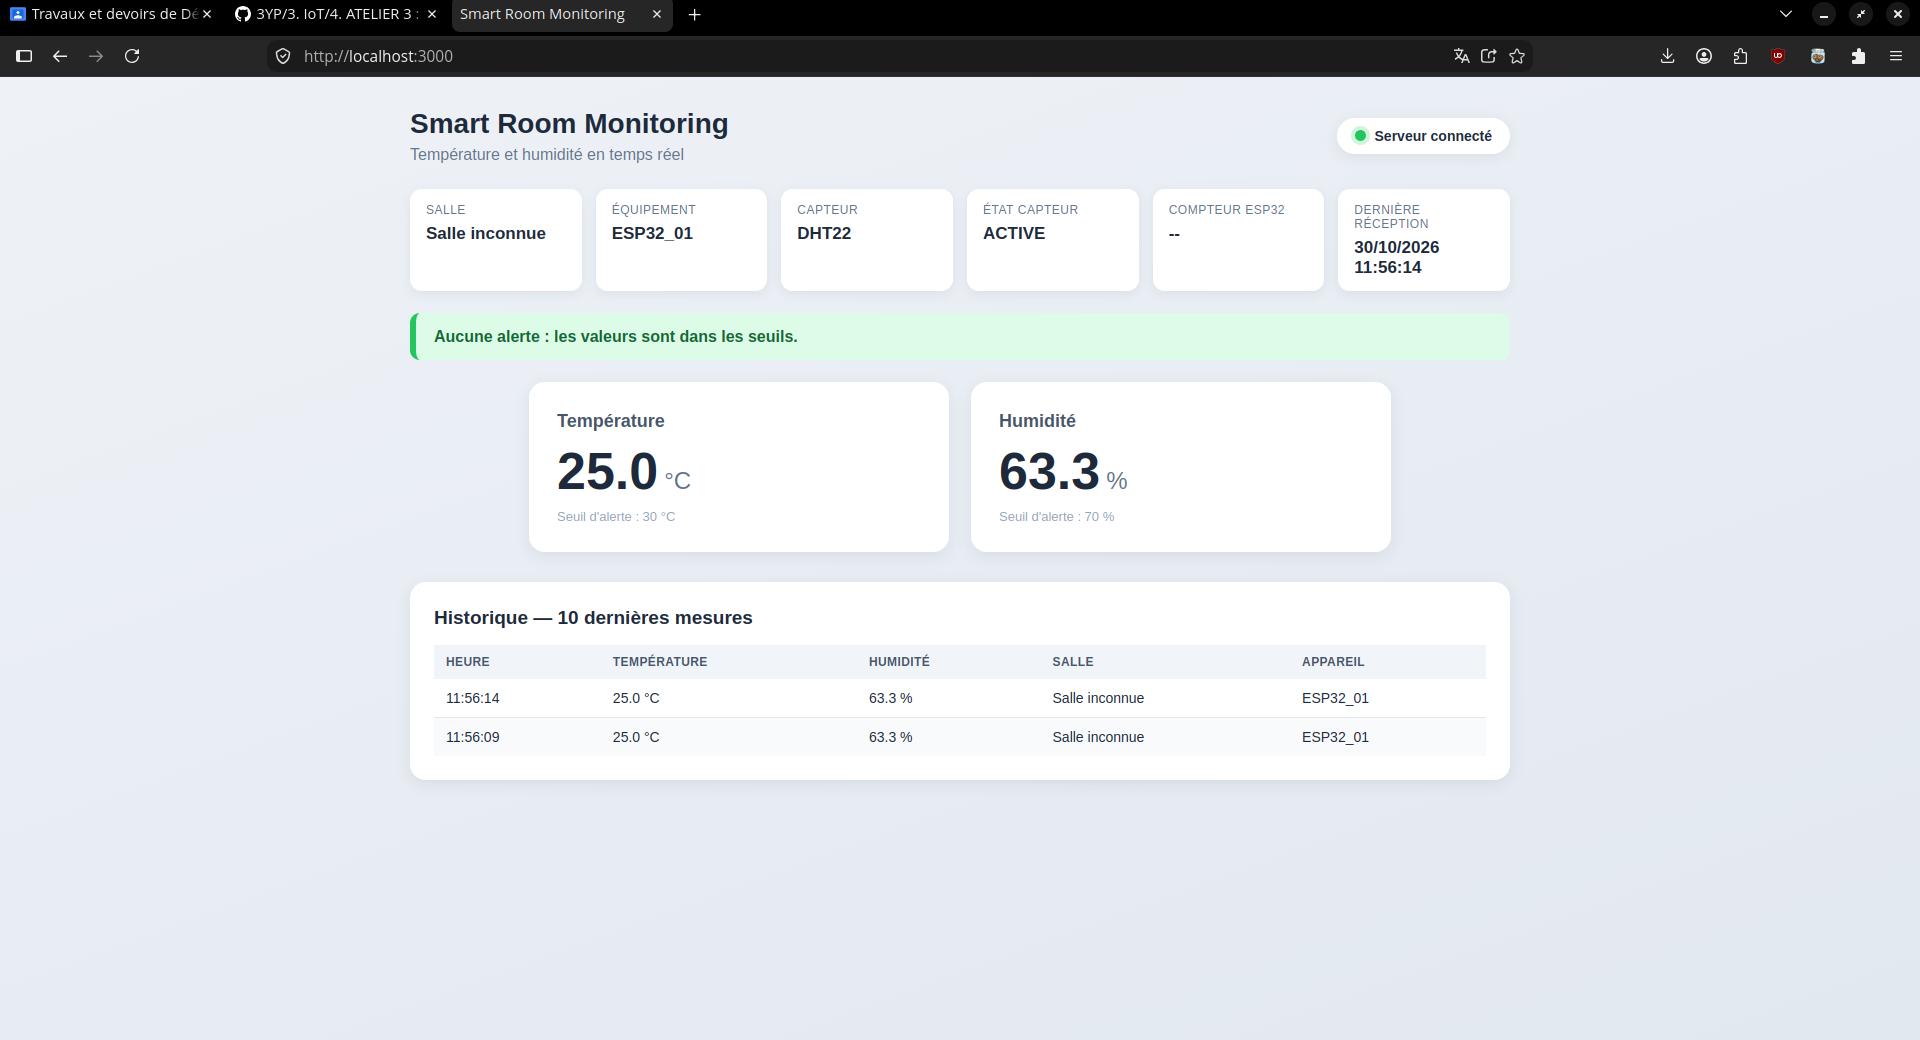
\includegraphics[width=0.98\textwidth]{dashboard.png}
\caption{Tableau de bord en fonctionnement : température 25,0~\textdegree C, humidité 63,3~\%, serveur connecté.}
\label{fig:dashboard}
\end{figure}

La capture montre une mesure à 25,0~\textdegree C et 63,3~\% d'humidité, avec la salle
\og Salle inconnue \fg{}, l'équipement \texttt{ESP32\_01}, le capteur \texttt{DHT22}, l'état
\texttt{ACTIVE} et un compteur à \texttt{--}. Ces valeurs illustrent le mécanisme de valeurs
par défaut décrit dans la partie 4 : le payload envoyé pendant l'essai ne contenait que
\texttt{device\_id}, \texttt{temperature} et \texttt{humidity}. La dernière réception est
horodatée au 30/10/2026 à 11:56:14, ce qui correspond à 10:56:14 UTC dans le journal serveur
(figure~\ref{fig:server}), le navigateur affichant l'heure locale (UTC+1).

\subsection{Logique cliente}

Le script client ouvre une connexion Socket.IO avec \texttt{io()}, écoute les événements
\texttt{newMeasurement} et \texttt{history}, puis met à jour le DOM. La fonction
\texttt{displayMeasurement} (code~\ref{lst:dashboard-js}) renseigne les cartes et déclenche
les alertes. Le tableau de bord utilise \texttt{toFixed(1)} pour afficher une décimale et
\texttt{toLocaleTimeString("fr-FR", \{hour12:false\})} pour un horodatage en 24~h.

\begin{lstlisting}[language=JavaScript,firstnumber=381,
  caption={Affichage d'une mesure et calcul des alertes (\texttt{nodeserver/public/dashboard.html}).},
  label={lst:dashboard-js}]
function applyAlerts(temperature, humidity) {
  const temperatureAlert = temperature > TEMPERATURE_THRESHOLD;
  const humidityAlert = humidity > HUMIDITY_THRESHOLD;

  document
    .getElementById("temperature-card")
    .classList.toggle("alert", temperatureAlert);

  document
    .getElementById("humidity-card")
    .classList.toggle("alert", humidityAlert);

  const alerts = [];

  if (temperatureAlert) {
    alerts.push(
      `Température trop élevée : ${temperature.toFixed(1)} °C ` +
      `(seuil : ${TEMPERATURE_THRESHOLD} °C)`
    );
  }

  if (humidityAlert) {
    alerts.push(
      `Humidité trop élevée : ${humidity.toFixed(1)} % ` +
      `(seuil : ${HUMIDITY_THRESHOLD} %)`
    );
  }

  const container = document.getElementById("alerts");

  if (alerts.length === 0) {
    container.innerHTML =
      '<div class="alert ok">Aucune alerte : les valeurs sont dans les seuils.</div>';
    return;
  }

  container.innerHTML = alerts
    .map((message) => `<div class="alert">⚠ ${message}</div>`)
    .join("");
}

function displayMeasurement(data) {
  const temperature = Number(data.temperature);
  const humidity = Number(data.humidity);

  document.getElementById("temperature").textContent = temperature.toFixed(1);
  document.getElementById("humidity").textContent = humidity.toFixed(1);

  document.getElementById("room").textContent = data.location || "--";
  document.getElementById("device").textContent = data.device_id || "--";
  document.getElementById("sensor").textContent = data.sensor_type || "--";
  document.getElementById("sensor-status").textContent = data.status || "--";
  document.getElementById("counter").textContent =
    data.counter !== undefined && data.counter !== null ? data.counter : "--";
  document.getElementById("time").textContent = formatDateTime(data.receivedAt);

  applyAlerts(temperature, humidity);
}
\end{lstlisting}

\subsection{Seuils et alertes}

Les seuils sont définis en tête de script : 30~\textdegree C pour la température et 70~\% pour
l'humidité (tableau~\ref{tab:alertes}). Ils sont volontairement simples et adaptés à une salle
de travaux pratiques ; ils pourraient être rendus configurables depuis l'interface.

\begin{table}[H]
\centering
\small
\begin{tabularx}{\textwidth}{@{}l l X@{}}
\toprule
Grandeur & Seuil & Comportement de l'interface \\
\midrule
Température & $> 30$~\textdegree C & Bordure rouge sur la carte et message d'alerte explicite. \\
Humidité & $> 70$~\% & Bordure rouge sur la carte et message d'alerte explicite. \\
Aucune alerte & valeurs dans les seuils & Bandeau vert \og Aucune alerte \fg{}. \\
\bottomrule
\end{tabularx}
\caption{Seuils d'alerte du tableau de bord.}
\label{tab:alertes}
\end{table}

Avec 25,0~\textdegree C et 63,3~\%, les deux grandeurs sont dans les seuils : la capture de la
figure~\ref{fig:dashboard} affiche donc le bandeau vert et aucune bordure rouge.

\subsection{Initialisation et reconnexion}

Au chargement, le script exécute deux requêtes en parallèle : \texttt{/api/measurements/latest}
et \texttt{/api/measurements/history}. Si l'historique est disponible, il est affiché et la
mesure la plus récente est utilisée pour remplir les cartes ; sinon, la dernière mesure est
affichée seule. Cette stratégie évite un écran vide après un rechargement de page.

Socket.IO gère automatiquement la reconnexion du navigateur. Les événements \texttt{connect}
et \texttt{disconnect} mettent à jour le badge ; lorsque la connexion revient, le serveur
renvoie l'état courant. Le client ne conserve pas de copie persistante des mesures : il
reconstruit son affichage à partir du serveur.

\subsection{Prévention des injections HTML}

Les champs provenant du serveur sont échappés avant insertion dans le tableau d'historique
grâce à la fonction \texttt{escapeHtml}. Cette précaution évite qu'un identifiant d'appareil
ou un nom de salle contenant du HTML ne soit interprété par le navigateur. Elle est
particulièrement importante si le système est un jour ouvert à des équipements tiers.

% ---------------------------------------------------------------------------
\section{Tests et résultats}
% ---------------------------------------------------------------------------

\subsection{Protocole de test}

Les essais ont été réalisés avec le matériel réel, dans l'ordre suivant :

\begin{enumerate}
  \item compilation et téléversement du firmware sur l'ESP32 ;
  \item ouverture du moniteur série à 115~200~bauds ;
  \item démarrage du serveur avec \texttt{node server.js}, puis vérification du message
        \og Serveur actif sur http://0.0.0.0:3000 \fg{} ;
  \item ouverture du tableau de bord à l'adresse \texttt{http://localhost:3000} ;
  \item observation pendant plusieurs minutes des trois interfaces : série, console serveur
        et navigateur ;
  \item tests complémentaires de validation avec des requêtes HTTP volontairement invalides.
\end{enumerate}

\subsection{Journal série de l'ESP32}

La figure~\ref{fig:serial} presente une première série d'envois. Chaque cycle affiche l'objet
JSON envoyé, puis la réponse du serveur et le code HTTP. Les valeurs de température restent à
24,8~\textdegree C ; l'humidité oscille entre 64,7~\% et 64,9~\%. La quasi-totalité des requêtes
reçoit un code 200, ce qui confirme la réception et le traitement correct des mesures.

\begin{figure}[H]
\centering
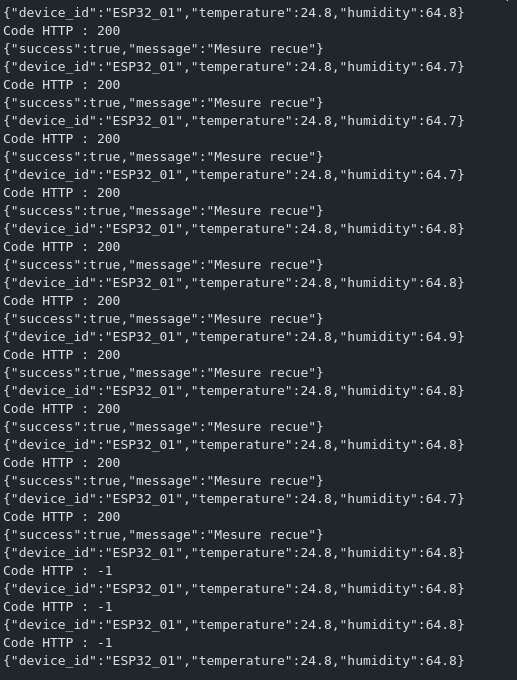
\includegraphics[width=0.56\textwidth]{serial.png}
\caption{Journal série de l'ESP32 : payloads JSON, réponses du serveur et codes HTTP.}
\label{fig:serial}
\end{figure}

En fin de série, plusieurs lignes affichent \texttt{Code HTTP : -1}. Ce code signifie que la
requête n'a pas abouti : le serveur était momentanément injoignable, ou la connexion Wi-Fi a
été interrompue. Le firmware se contente alors de journaliser l'échec et de poursuivre ; il ne
réessaie pas. Cette observation justifie l'ajout d'une politique de reconnexion et d'un
stockage local tampon dans une version ultérieure.

\subsection{Journal du serveur}

La figure~\ref{fig:server} montre le journal du serveur pendant une seconde série. On y lit le
message de démarrage, la connexion d'un tableau de bord, puis des objets \texttt{Mesure recue}
contenant les champs normalisés et l'horodatage \texttt{receivedAt}. Les mesures sont reçues
toutes les cinq secondes environ : 10:56:09, 10:56:14, 10:56:19, 10:56:24 et 10:56:29 UTC.

\begin{figure}[H]
\centering
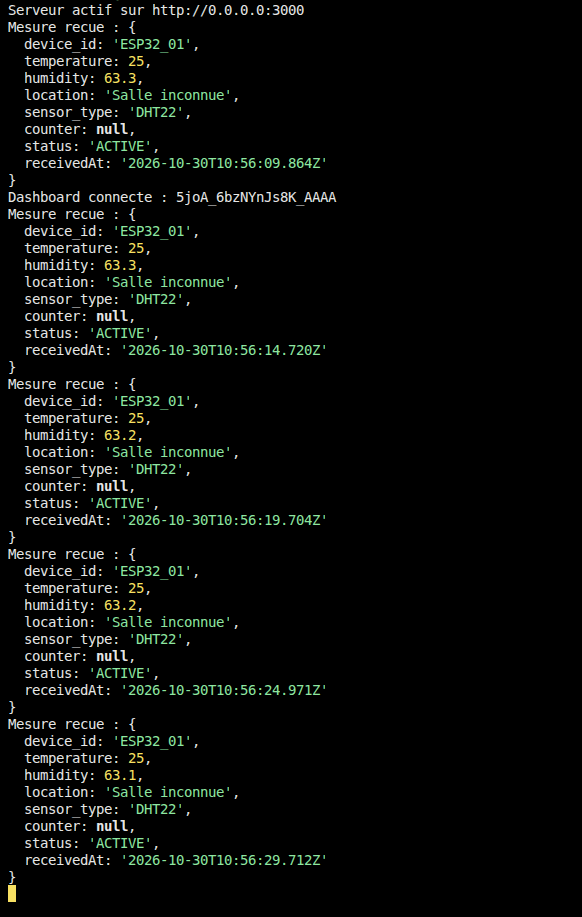
\includegraphics[width=0.56\textwidth]{server.png}
\caption{Journal du serveur Node.js : démarrage, connexion du dashboard et mesures reçues.}
\label{fig:server}
\end{figure}

Les valeurs de cette série sont stables : 25~\textdegree C et une humidité qui décroît
lentement de 63,3~\% à 63,1~\%. La présence de \texttt{location: 'Salle inconnue'} et de
\texttt{counter: null} confirme que le payload de test ne contenait que les trois champs
minimaux : le serveur a appliqué ses valeurs par défaut, comme prévu par le code.

\subsection{Tableau de bord en fonctionnement}

La figure~\ref{fig:dashboard} montre l'interface au même moment. Le badge \og Serveur
connecté \fg{} est vert, la dernière réception affiche 11:56:14 (heure locale) et l'historique
présente les mesures avec leur heure, leur température, leur humidité, leur salle et leur
appareil. L'affichage est cohérent avec le journal serveur : 10:56:14 UTC correspond bien à
11:56:14 en UTC+1.

\subsection{Synthèse des mesures}

Le tableau~\ref{tab:mesures} reprend les cinq mesures de la seconde série, avec l'écart entre
deux réceptions successives. La période moyenne est de 4,96~s, proche de l'intervalle de 5~s
programmé dans le firmware.

\begin{table}[H]
\centering
\small
\begin{tabular}{@{}c c c r r r@{}}
\toprule
\# & Heure UTC & Heure locale & Température (\textdegree C) & Humidité (\%) & Écart (s) \\
\midrule
1 & 10:56:09,864 & 11:56:09 & 25,0 & 63,3 & --- \\
2 & 10:56:14,720 & 11:56:14 & 25,0 & 63,3 & 4,86 \\
3 & 10:56:19,704 & 11:56:19 & 25,0 & 63,2 & 4,98 \\
4 & 10:56:24,971 & 11:56:24 & 25,0 & 63,2 & 5,27 \\
5 & 10:56:29,712 & 11:56:29 & 25,0 & 63,1 & 4,74 \\
\bottomrule
\end{tabular}
\caption{Mesures de la seconde série et intervalles de réception.}
\label{tab:mesures}
\end{table}

\begin{figure}[H]
\centering
\begin{tikzpicture}
\begin{axis}[
  width=0.86\textwidth,
  height=5.6cm,
  xlabel={Temps écoulé depuis la première mesure (s)},
  ylabel={Humidité relative (\%)},
  xmin=-1, xmax=22,
  ymin=62.9, ymax=63.5,
  xtick={0,5,10,15,20},
  ytick={63.0,63.1,63.2,63.3,63.4},
  yticklabel style={/pgf/number format/use comma},
  grid=major,
  grid style={draw=coverblue!12},
  axis line style={draw=coverblue!60},
  tick style={draw=coverblue!60},
  mark=*,
  mark size=2.2pt,
  line width=0.9pt,
  color=teal,
  legend style={draw=none,fill=none,font=\small,at={(0.02,0.98)},anchor=north west}
]
\addplot coordinates {(0,63.3) (4.856,63.3) (9.840,63.2) (15.107,63.2) (19.848,63.1)};
\addlegendentry{Humidité mesurée}
\end{axis}
\end{tikzpicture}
\caption{Évolution de l'humidité pendant la seconde série ; la température reste constante à 25,0~\textdegree C.}
\label{fig:humidite}
\end{figure}

La température est parfaitement stable sur cette série, tandis que l'humidité diminue de
0,2 point. Cette variation reste faible et cohérente avec un capteur de classe bas coût. Les
écarts entre réceptions (4,74 à 5,27~s) s'expliquent par la latence réseau, le temps de
traitement du serveur et l'arrondi des horodatages ; ils restent compatibles avec une
acquisition toutes les cinq secondes.

\subsection{Tests de validation}

Des requêtes invalides ont été envoyées avec \texttt{curl} pour vérifier le comportement du
serveur. Le tableau~\ref{tab:tests} résume les cas testés et le code~\ref{lst:api-errors}
donne le corps des réponses obtenues ; toutes portent le code HTTP 400.

\begin{table}[H]
\centering
\small
\begin{tabularx}{\textwidth}{@{}p{3.4cm} X p{1.7cm}@{}}
\toprule
Cas & Donnée envoyée & Code \\
\midrule
\texttt{device\_id} absent & \texttt{\{"temperature":24.8,"humidity":64.7\}} & 400 \\
Température non numérique & \texttt{"temperature":"chaud"} & 400 \\
Humidité hors plage & \texttt{"humidity":120} & 400 \\
\bottomrule
\end{tabularx}
\caption{Cas de validation testés.}
\label{tab:tests}
\end{table}

\begin{lstlisting}[language=JavaScript,caption={Corps des réponses HTTP 400 renvoyées par le serveur.},label={lst:api-errors},aboveskip=4pt,belowskip=4pt]
{"success":false,"message":"Donnees invalides",
 "errors":["device_id est obligatoire et doit etre une chaine de caracteres"]}
{"success":false,"message":"Donnees invalides",
 "errors":["temperature doit etre un nombre"]}
{"success":false,"message":"Donnees invalides",
 "errors":["humidity doit etre comprise entre 0 et 100 %"]}
\end{lstlisting}

\enlargethispage{3\baselineskip}
Les trois requêtes sont rejetées avec un code 400 et un message explicite. Aucune mesure
invalide n'est ajoutée à l'historique, car le contrôle précède la construction de l'objet
\texttt{measurement}.


\end{document}
